\chapter{Implementacja modelu programowego}
Pierwszym zadaniem było stworzenie modeli programowych algorytmów MeanShift oraz Hog+SVM, bez warstwy nadzorującej/sterującej dronem. Wybrano środowisko MATLAB ze względu na jego powszechne zastosowanie w branży naukowej/inżynierskiej, co skutkuje olbrzymią bazą bibliotek i materiałów pomocniczych. W tym przypadku MATLAB ułatwia pracę na obrazach lub sekwencjach wideo poprzez: wczytywanie materiału, wyświetlanie, dostęp do poszczególnych klatek oraz zapewnia wiele wbudowanych funkcji, m.in. do konwersji określonych przestrzeni barw oraz obliczania maszyny wektorów nośnych.

\section{Model MeanShift}

Skrypt rozpoczyna działanie od wyznaczenia jądra obszaru o wymiarach $100 \times 100$ oraz jego gradientów. Po tym następuje właściwa część algorytmu, która pracuje na wczytanym materiale wideo, przekonwertowanym do przestrzeni HSV. Obszarem śledzonym jest kwadrat $100\times 100$, który dla pierwszej klatki obrazu jest zlokalizowany w miejscu startowym ramki $1280\times 720$ pikseli. Dla tego fragmentu obliczany jest histogram barw. Wczytując kolejne klatki, algorytm oblicza histogram kandydatów ostatecznie zestawiając go z oryginalnym i wyznaczając przesunięcie w pionie i poziomie. Dla każdej z klatek operacja ta jest przeprowadzana 10 razy, poprawiając precyzję ostatecznego przesunięcia. Przed rozpoczęciem przetwarzania kolejnej klatki, następuje aktualizacja pozycji obszaru. Po wykonaniu algorytmu dla zdefiniowanej liczbie klatek, skrypt wyświetla film w oryginalnych barwach RGB z dorysowaną czerwoną ramką otaczającą śledzony obszar, co pozwala wizualnie sprawdzić poprawność działania całego kodu. Niestety, czas wykonania tej symulacji jest nieporównywalnie dłuższy od rzeczywistego trwania sekwencji i, przykładowo, na komputerze wyposażonym w procesor klasy i7 materiał o długości 685 klatek (ok. 11 sekund filmu) jest przetwarzany w czasie ok. 100 sekund.

Rysunek \ref{fig:meanshift_prog} przedstawia śledzenie obiektu będącego czerwoną koszulką z ciemnym poziomym paskiem. Kolejne zrzuty są realizowane z odstępem 100 klatek.
 
\begin{figure}[]
	\centering
	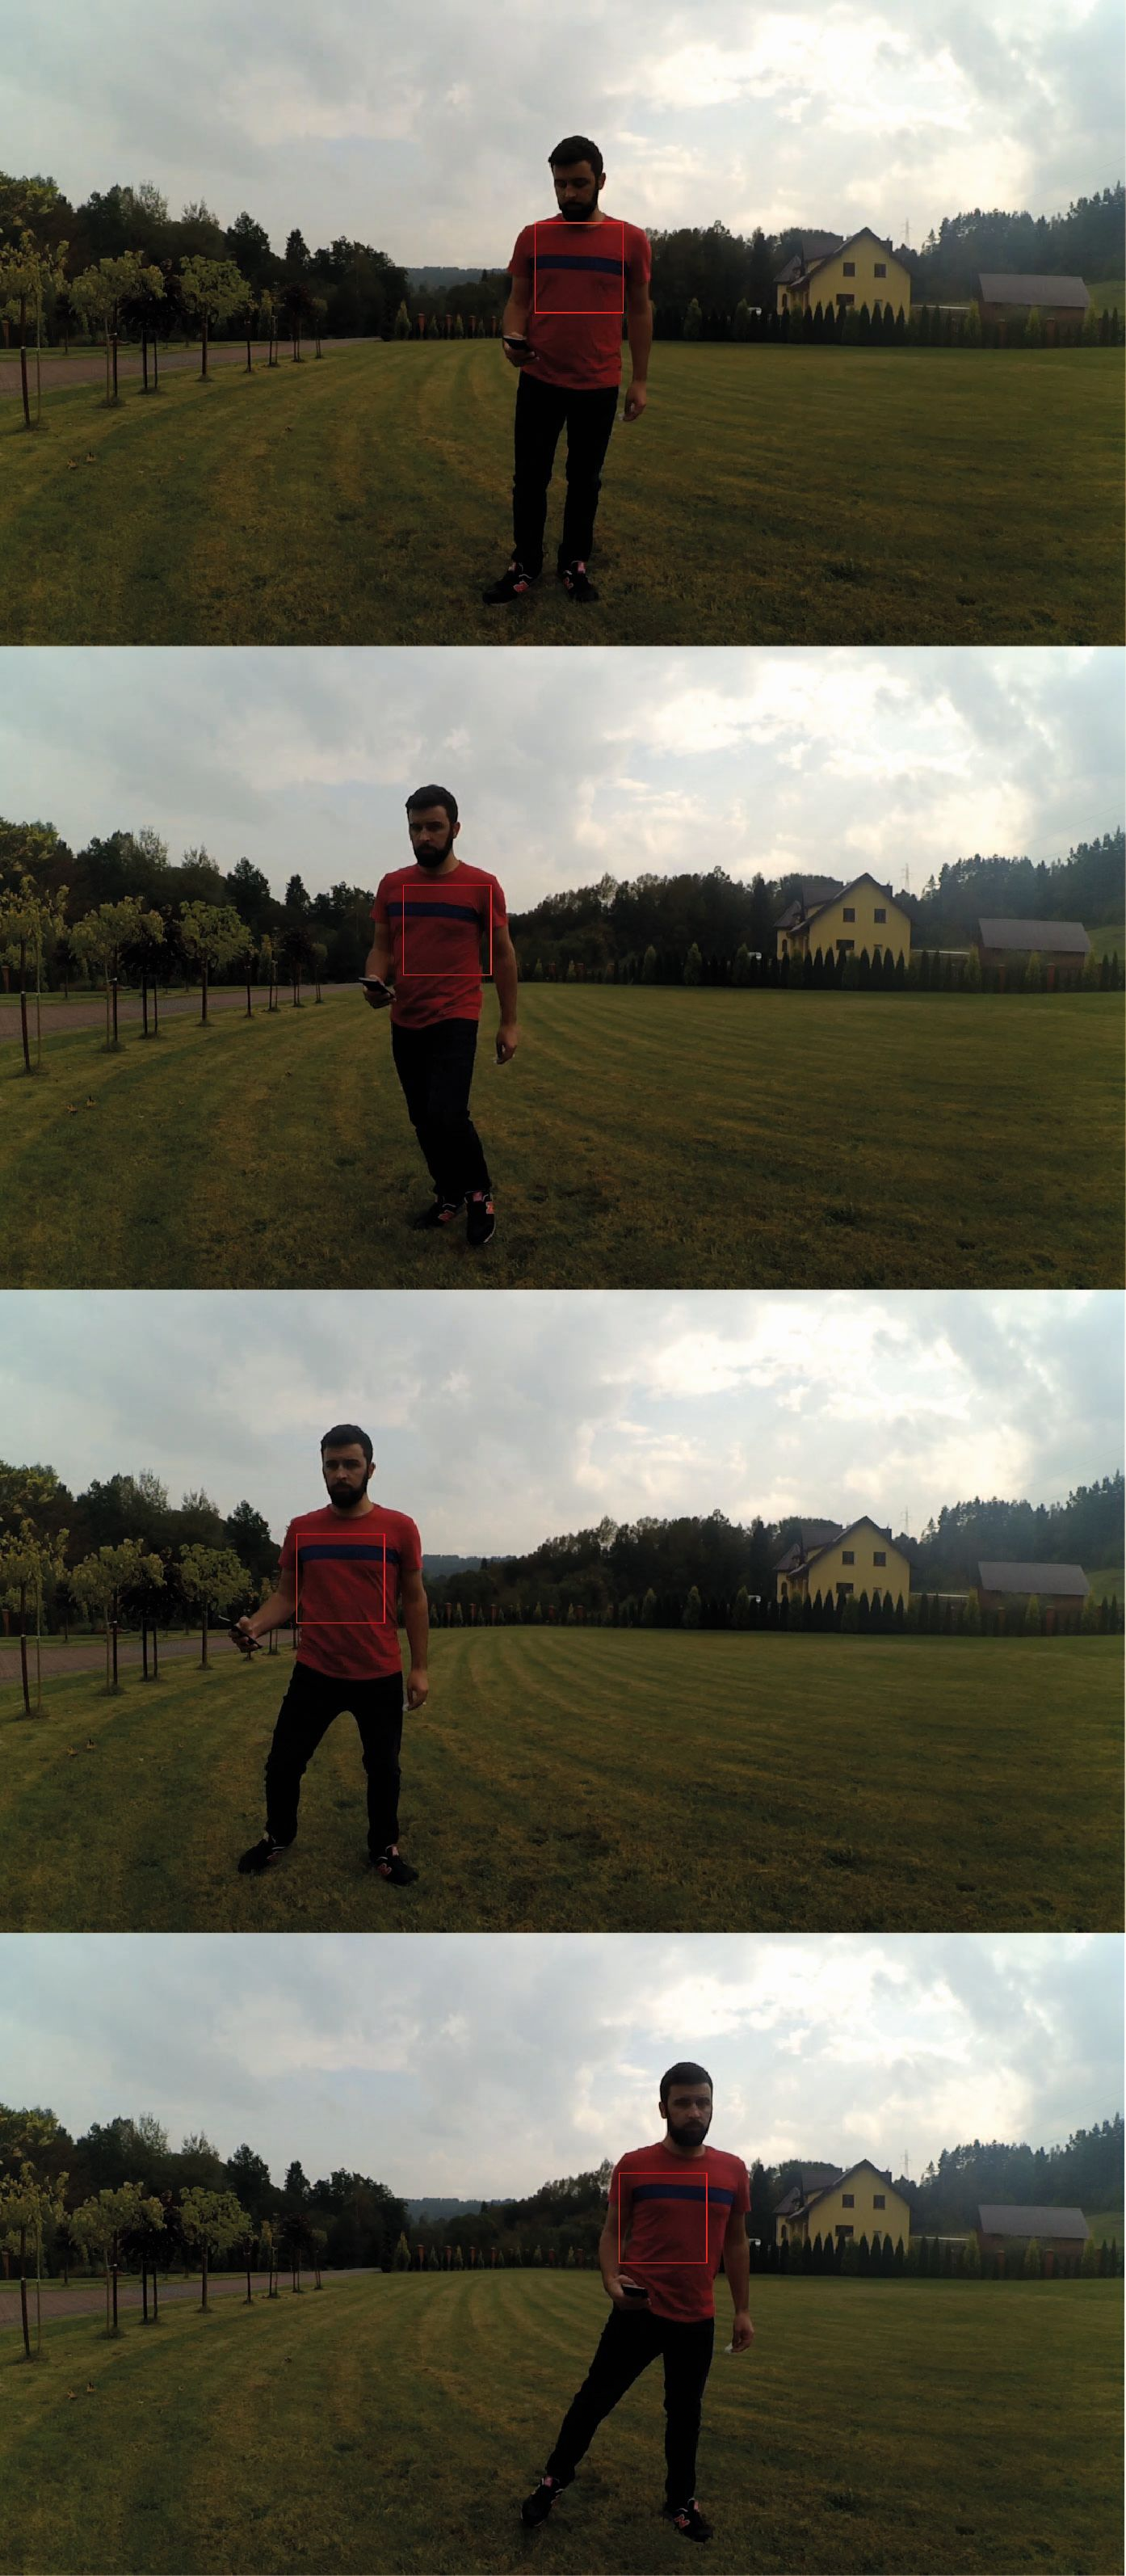
\includegraphics[width=10cm]{3_meanshift.jpg}
	\caption{Śledzenie MeanShift}
	\label{fig:meanshift_prog}
\end{figure}

\section{Model HoG+SVM}

Głównym zadaniem modelu programowego jest próba znalezienia osoby w przeskalowanym obrazie, bazując na obszarze wokół wprowadzonych współrzędnych punktu środkowego.

Działanie skryptu rozpoczyna się od przeprowadzenia sekwencji uczenia klasyfikatora, która bazuje na dwóch tablicach: jedna agreguje wektory cech, a druga przechowuje skojarzone z nimi klasy (0 lub 1). Wykorzystywana baza obrazów wyposażona jest w pliki z ich listami (osobno dla pozytywnych i negatywnych przykładów), co umożliwia proste wczytywanie kolejnych próbek. Oczekuje się tu rozmiaru $128\times 64$ pikseli, jednak niektóre (zwłaszcza negatywne) obrazy są za duże - przeprowadza się tutaj wycięcie fragmentu o podanym wyżej rozmiarze ze środka każdej próbki. Kolejnymi etapami dla takiego obszaru są kolejno: konwersja do odcieni szarości oraz obliczenie wektora cech. Ten proces przeprowadzono zgodnie z informacjami zawartymi w \ref{sec:HOG&SVM}; za normę blokową obrano L2 (\ref{eq:HOG_norm3}), natomiast rozmiar komórki to $4\times 4$ piksele. Po przetworzeniu każdego obrazu dopisuje się wektor cech oraz klasę do odpowiednich tablic.
\newline
Gotowe zestawy danych stanowią parametry dla wbudowanej w MATLABa funkcji \textit{svmtrain}, która zwraca strukturę \textit{svm\char`_struct} z parametrami wykorzystywanymi potem przez klasyfikator.

Opisany powyżej proces ma powtarzalne wyniki. Jest jednorazowy, lecz także dość czasochłonny - dlatego nie ma potrzeby przeprowadzać go niepotrzebnie (skrypt sprawdza obecność zmiennej \textit{svm\char`_struct} i dopiero w przypadku jego braku przeprowadzi uczenie).

Właściwa część skryptu rozpoczyna się od wczytania obrazu wejściowego. O jego odpowiednim przeskalowaniu decyduje parametr ustawiany przed rozpoczęciem działania. W ten sposób zdefiniowane są również współrzędne środka obszaru detekcji. Kolejnym krokiem jest obliczenie $5\times 9$ wektorów cech na fragmencie $144 \times 96$ - widoczna różnica w podejściu względem procesu uczenia wynika z planu znalezienia jak najlepszego wyniku detekcji w danym obszarze. Idąc za przykładem wbudowanej w MATLAB funkcji \textit{svmclassify}, następuje klasyfikacja każdego obliczonego wektora cech. Końcowym etapem jest wyświetlenie przeskalowanego obrazu w kolorze, z naniesionym konturem o wymiarach $128\times 64$ otaczającym obszar najlepszej detekcji. 

Przykłady zaprezentowano poniżej, gdzie analizie poddano fragment o środku w pozycji $\{640,360\}$.
Różowym konturem oznaczono okno detekcji $144 \times 96$, natomiast na czerwono zakreślono ostateczne obszary $128\times 64$ pozytywnie wybrane przez klasyfikator. Przedstawiono również tabelę z wynikami.
\begin{figure}[]
	\centering
	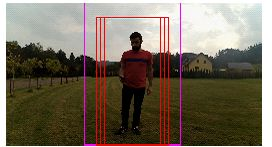
\includegraphics[width=10cm]{3_SVM_model.jpg}
	\caption{Detekcja na oknie wewnątrz obrazu (skala: 5)}
	\label{fig:SVMmodel}
\end{figure}

\newcolumntype{P}[1]{>{\centering\arraybackslash}p{#1}}
\begin{table}[]
	\centering
	\begin{tabular}{|P{1.2cm} |P{1.2cm} |P{1.2cm} |P{1.2cm} |P{1.2cm} |P{1.2cm} |P{1.2cm} |P{1.2cm} |P{1.2cm} |}
		
		\hline
$1.4357$ &   $1.0343$  &  $1.4887$  &  $1.1960$  &  $1.1270$  &  $1.2742$ &   $0.6366$  &  $0.9465$  &  $0.8936$ \\ \hline
$0.9876$ &   $1.1790$  &  $1.7361$  &  $1.4707$  &  $1.0850$  &  $1.2012$ &   $1.2482$  &  $1.5096$  &  $1.2834$ \\ \hline
$1.4188$ &   $1.3449$  &  $2.1487$  &  $1.8528$  &  $0.9389$  &  $0.7458$ &   $1.0194$  &  $1.5121$  &  $1.7702$ \\ \hline
$1.5967$ &   $2.0461$  &  $1.7974$  &  $1.1585$  &  $0.6553$  &  $0.6955$ &   $0.5781$  &  $1.6717$  &  $1.3235$ \\ \hline
$1.2971$ &   $2.0113$  &  $1.2289$  & $\textbf{-0.0191}$  & $\textbf{-0.5477}$  & $\textbf{-1.0460}$ &   $0.2423$  &  $1.0235$  &  $1.7798$ \\ \hline		
	\end{tabular}
	\caption{Tabela z wynikami dla $5 \times 9$ detekcji z rysunku \ref{fig:SVMmodel}}
	\label{tab:scale_window_cover_5}
\end{table}

\begin{figure}[h]
	\centering
	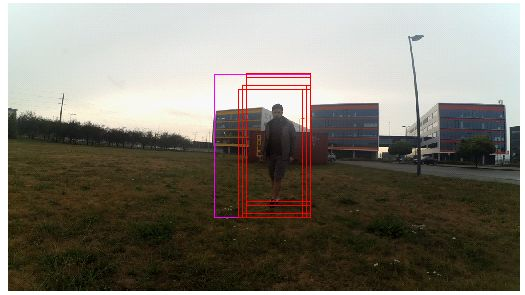
\includegraphics[width=16cm]{3_SVM_model_2_5.jpg}
	\caption{Detekcja na oknie wewnątrz obrazu (skala: 2.5)}
	\label{fig:SVMmodel_2_5}
\end{figure}

\newcolumntype{P}[1]{>{\centering\arraybackslash}p{#1}}
\begin{table}[h]
	\centering
	\begin{tabular}{|P{1.2cm} |P{1.2cm} |P{1.2cm} |P{1.2cm} |P{1.2cm} |P{1.2cm} |P{1.2cm} |P{1.2cm} |P{1.2cm} |}
		
		\hline
    $2.1223$  &  $1.9234$  &  $1.8072$ & $1.8854$  &  $1.6932$ &  $1.5320$  & $ 0.5443$ &  $ 0.2648$  & $\textbf{-0.0366}$ \\ \hline
$1.9547$  &  $2.5649$  &  $1.6400$ & $1.7075$  &  $1.1940$ &  $1.5821$  & $ 0.6492$ &  $ 0.2804$  & $\textbf{-0.0880}$ \\ \hline
$2.5165$  &  $2.7328$  &  $2.3592$ & $2.2650$  &  $2.1196$ &  $1.1509$  & $ 0.8788$ &  $ 0.6314$  & $ 0.1222$ \\ \hline
$2.4744$  &  $2.8618$  &  $2.7310$ & $2.6338$  &  $2.1627$ &  $1.4763$  & $ 0.4520$ &  $\textbf{-0.7166}$  & $\textbf{-1.1757}$ \\ \hline
$2.6806$  &  $2.4200$  &  $2.2032$ & $1.6812$  & $1.9216$ &  $0.9355$  & $\textbf{-0.0505}$ &  $\textbf{-1.3537}$  & $\textbf{-1.3712}$ \\ \hline	
	\end{tabular}
	\caption{Tabela z wynikami dla $5 \times 9$ detekcji z rysunku \ref{fig:SVMmodel_2_5}}
	\label{tab:scale_window_cover_2_5}
\end{table}

\begin{figure}[h]
	\centering
	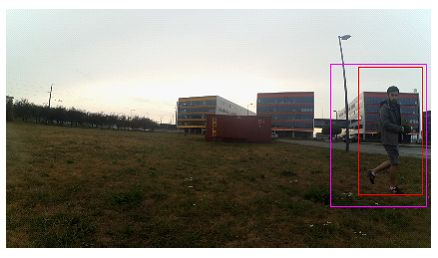
\includegraphics[width=16cm]{3_SVM_model_3.jpg}
	\caption{Detekcja na oknie wewnątrz obrazu (skala: 3)}
	\label{fig:SVMmodel_3}
\end{figure}


\newcolumntype{P}[1]{>{\centering\arraybackslash}p{#1}}
\begin{table}[h]
	\centering
	\begin{tabular}{|P{1.2cm} |P{1.2cm} |P{1.2cm} |P{1.2cm} |P{1.2cm} |P{1.2cm} |P{1.2cm} |P{1.2cm} |P{1.2cm} |}
	\hline	
    $1.8159$  &  $1.8308$  &  $1.7164$  &  $1.4868$  &  $1.1955$  &  $1.1542$  &  $0.8346$  & $ 0.4625$   & $0.6144$ \\ \hline
$2.3357$  &  $2.6091$  &  $2.0017$  &  $2.0776$  &  $2.2638$  &  $1.8270$  &  $0.6915$  & $\textbf{-0.0323}$  &  $0.6554$ \\ \hline
$2.3233$  &  $2.4182$  &  $1.9292$  &  $2.1127$  &  $1.8924$  &  $1.7307$  &  $0.8044$  & $ 0.3019$  &  $0.7611$ \\ \hline
$1.5705$  &  $1.6276$  &  $1.5120$  &  $1.7848$  &  $1.6619$  &  $1.7323$  &  $0.4511$  & $ 0.8625$  &  $1.1717$ \\ \hline
$1.4874$  &  $1.8153$  &  $1.0768$  &  $1.2884$  &  $1.0186$  &  $1.8310$  &  $0.8986$  & $ 0.6349$  &  $1.1386$ \\ \hline
	\end{tabular}
	\caption{Tabela z wynikami dla $5 \times 9$ detekcji z rysunku \ref{fig:SVMmodel_3}}
	\label{tab:scale_window_cover_3}
\end{table}